\subsubsection{The stationary Richardson method}\label{subsubsection: The stationary Richardson method}

The stationary Richardson method is a way of refining a guess for solving the general problem $Ax = b$. We \textbf{start with an initial guess for the solution}, then we \textbf{keep adjusting that guess based on how far it is from the actual answer}. The \textbf{adjustments depend on a parameter we choose}, which can speed up or slow down how quickly we get to the right answer. We \textbf{keep doing this until our guess is close enough to the actual solution}.

\highspace
Mathematically, given $\mathbf{x}^{\left(0\right)} \in \mathbb{R}^{n}$, $\alpha \in \mathbb{R}$, the stationary Richardson method is based on the following recursive update:
\begin{equation}\label{eq: stationary richardson x calcolus}
    \mathbf{x}^{\left(k+1\right)} = \mathbf{x}^{\left(k\right)} + \alpha \cdot \underbrace{\left(\mathbf{b} - A\mathbf{x}^{\left(k\right)}\right)}_{\text{residual }\mathbf{r}^{\left(k\right)}}
\end{equation}
The idea is to update the numerical solution by adding a quantity proportional to the residual. Indeed, it is expected that if the residual is \emph{large} (\emph{small}), the solution at step $k$ should be corrected \emph{much} (\emph{little}). Where $\alpha$ is a weighted version of the residual.
\begin{itemize}
    \item Iteration matrix $B_{\alpha}$:
    \begin{equation*}
        B_{\alpha} = I - \alpha A
    \end{equation*}
    \item $\mathbf{f}$:
    \begin{equation*}
        \mathbf{f} = \alpha \mathbf{b}
    \end{equation*}
\end{itemize}
We now ask ourselves \textbf{which value of the parameter} $\alpha$, among those that \textbf{guarantee convergence}, \textbf{maximizes the speed of convergence}. We introduce the following $A$-induced norm where A is SPD:
\begin{equation*}
    {\left|\left|\mathbf{z}\right|\right|}_{A} = \sqrt{
        \displaystyle\sum_{i,j = 1}^{n} a_{ij}z_{i}z_{j}
    }
    \iff
    {\left|\left|\mathbf{z}\right|\right|}_{A} = \sqrt{\left(A\mathbf{z}, \mathbf{z}\right)} = \sqrt{\mathbf{z}^{T} A \mathbf{z}}
\end{equation*}
We look for $0 < \alpha_{\text{opt}} < \dfrac{2}{\lambda_{\max\left(A\right)}}$ such that $\rho\left(B_{\alpha}\right)$ is minimum. That is:
\begin{equation*}
    \alpha_{\text{opt}} = \underset{0 < \alpha < \frac{2}{\lambda_{\max\left(A\right)}}}{\mathrm{argmin}} \left\{\underset{i}{\max} \left|1 - \alpha\lambda_{i}\left(A\right)\right|\right\}
\end{equation*}
To understand which $\alpha$ to choose, we plot the problem. On the \emph{x-axis} are the values of $\alpha$ and on the \emph{y-axis} is the spectral radius equal to $\left|1-\alpha\lambda_{i}\left(A\right)\right|$, with $i = 1, \dots, n$.

\highspace
In the figure \ref{fig: alpha stationary Richardson method} we can see that the upper bound of the spectral radius is equal to 1 (no convergence). Each line represents the possible value of the spectral radius for different values of $\alpha$. In \textbf{green} we see the \textbf{spectral radius equal to} $\rho\left(B_{\alpha}\right)$; it is important because its intersection with the upper bound of $\rho$ represents the right bound of the interval where the \textbf{values of $\alpha$ guarantee convergence}. It can also be seen by the \textbf{red arrow}. The \textbf{lowest point of the curve is where the spectral radius is minimized, indicating the best $\alpha$ for convergence}.

\highspace
In other words, the optimal value is given by the intersection between the curves:
\begin{equation*}
    \left|1 - \alpha \lambda_{1}\left(A\right)\right|
    \cap
    \left|1 - \alpha \lambda_{n}\left(A\right)\right|
\end{equation*}
That gives us the perfect formula:
\begin{equation}
    \alpha_{\text{opt}} = \dfrac{2}{\lambda_{\min}\left(A\right) + \lambda_{\max}\left(A\right)}
\end{equation}
\begin{figure}[!htp]
    \centering
    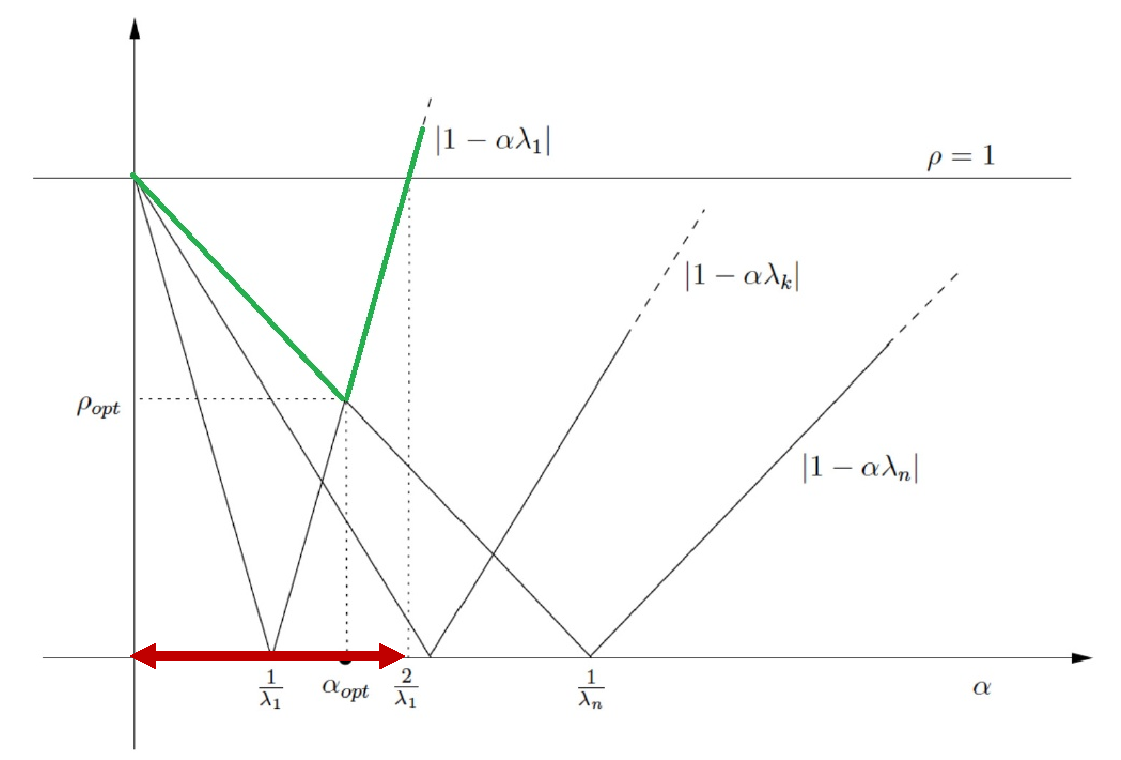
\includegraphics[width=\textwidth]{img/richardson-alpha-opt-1.pdf}
    \caption{Graphical representation of the optimal alpha to choose in the stationary Richardson method.}
    \label{fig: alpha stationary Richardson method}
\end{figure}

\noindent
If A is SPD, the eigenvalues of $A$ (real and positive) are:
\begin{equation*}
    \lambda_{\max}\left(A\right) = \lambda_{1}\left(A\right) \ge \lambda_{2}\left(A\right) \ge \cdots \ge \lambda_{n}\left(A\right) = \lambda_{\min}\left(A\right) > 0
\end{equation*}
\begin{theorem}
    Let A be a symmetric and positive definite matrix. The \textbf{stationary Richardson method is convergent if and only if}:
    \begin{equation}
        0 < \alpha < \dfrac{2}{\lambda_{\max}\left(A\right)}
    \end{equation}
\end{theorem}

\noindent
Since there is a strong correlation between the optimal $\alpha$ and the optimal spectral radius, we can obtain
\begin{equation*}
    \begin{array}{rcl}
        \rho_{\text{opt}} &=& \rho\left(B_{\alpha_{\text{opt}}}\right) \\ [.3em]
        &=& -1+\alpha_{\text{opt}}\lambda_{\max}\left(A\right) \\ [.3em]
        &=& 1-\alpha_{\text{opt}}\lambda_{\min}\left(A\right) \\ [.3em]
        &=& \dfrac{
            \lambda_{\max}\left(A\right) - \lambda_{\min}\left(A\right)
        }{
            \lambda_{\max}\left(A\right) + \lambda_{\min}\left(A\right)
        }
    \end{array}
\end{equation*}
Finally, since $A$ is SPD, we have the Euclidean norm equal to the maximum eigenvalue of A: ${\left|\left|A\right|\right|}_{2} = \lambda_{\max}\left(A\right)$. Moreover, $\lambda_{i}\left(A^{-1}\right) = \frac{1}{\lambda_{i}\left(A\right)}$, $i = 1, \dots, n$:
\begin{equation}\label{eq: optimal sepctral radius}
    \rho_{\text{opt}} = \dfrac{
        K\left(A\right)-1
    }{
        K\left(A\right)+1
    }
\end{equation}

\begin{flushleft}
    \textcolor{Green3}{\faIcon{tools} \textbf{Algorithm}}
\end{flushleft}
\begin{enumerate}
    \item \textbf{Start with an initial guess} $x^{\left(0\right)}$ and \textbf{select a parameter} $\alpha$.
    \item \textbf{Iteration}. For each $k$ calculate the value of the equation \ref{eq: stationary richardson x calcolus}.
    \item \textbf{Repeat until the changes are less than a specified tolerance}.
\end{enumerate}

\highspace
\begin{flushleft}
    \textcolor{Red2}{\faIcon{dollar-sign} \textbf{How much does it cost?}}
\end{flushleft}
The cost of each iteration depends by type of matrix:
\begin{itemize}
    \item \textbf{Dense matrix}: the cost of each iteration is about $n^{2}$ \textbf{operations}, where $n$ is the number of unknowns in the linear system.
    \item \textbf{Sparse matrix}: the cost of each iteration is only about $n$ \textbf{operations}.
\end{itemize}

\highspace
\begin{flushleft}
    \textcolor{Green3}{\faIcon{network-wired} \textbf{Can it be parallelized?}}
\end{flushleft}
The stationary Richardson method is not as easily parallelizable as the Jacobi method. Richardson uses the entire solution vector from the previous iteration in each step. This dependency makes it \textbf{more difficult to parallelize}.